\section{Scheduling with Unknown Arrival Types: The Nested WAIT Algorithm}
\label{sec:nested_wait}

The WAIT algorithm achieves near-optimal throughput when we know prompt types at arrival. In practice, however, we cannot predict how many tokens a prompt will generate—output lengths reveal themselves only as decode progresses. The \textit{Nested Waiting for Accumulated Inference Threshold} (Nested WAIT) algorithm exploits this gradual revelation: \textbf{prompts classify themselves on-the-fly} as they decode. Short prompts complete early and exit; longer prompts naturally advance to later segments. \textbf{No prediction is needed}—the algorithm simply lets each prompt reveal its type through its decode trajectory.

\begin{example}[Unknown Output Lengths]
\label{ex:unknown_output}
Continuing Example~\ref{ex:fcfs_cascade}, suppose output lengths are now \emph{unknown} at arrival: each ``Hello'' prompt receives either ``Hi'' (1 token) or ``Hi there!'' (2 tokens). The scheduler faces a dilemma. If it optimistically assumes all outputs are short (1 token each), it admits 6 prompts with capacity $C=12$, requiring $6 \times 2 = 12$ units after decode. But if some outputs turn out to be 2 tokens (requiring 3 units each), memory overflows and eviction cascades begin. Conversely, if the scheduler conservatively assumes all outputs are long, it admits only 4 prompts to stay safe, wasting 25\% of capacity when most outputs are actually short.

This dilemma---optimism leads to eviction, pessimism wastes capacity---leads to our design principles: (i) \emph{avoid eviction} by not over-committing memory; (ii) \emph{classify on-the-fly} by letting prompts reveal their type as they decode; (iii) \emph{don't waste throughput} by exploiting available capacity; (iv) \emph{let shorter prompts finish first} so they free memory without being blocked by longer ones.
\end{example}

\subsection{Algorithm Overview}

Example~\ref{ex:unknown_output} reveals a fundamental dilemma: optimism risks eviction, pessimism wastes capacity. We resolve this through on-the-fly classification. Rather than predicting output lengths at arrival, Nested WAIT lets prompts reveal their output as they decode. Short prompts complete early and exit; longer prompts naturally advance to later segments.

The core idea is \textbf{nested thresholds}: segment 1 handles all prompts from decode stage 0 to $l_1'$; segment 2 handles prompts that survive past $l_1'$ (i.e., types 2 through $m$); segment 3 handles prompts past $l_2'$; and so on. Each segment $k$ has its own threshold $n_k$ controlling when it processes prompts. This nesting achieves two goals: (i) short prompts complete in early segments without being blocked by long prompts; (ii) each segment operates at high memory utilization for its remaining types.

Formally, let output lengths satisfy $l_1' < l_2' < \dots < l_m'$, where type $j$ has decode length $l_j'$. We organize inference into $m$ nested segments, where segment $k$ spans decode stages from $l_{k-1}' + 1$ to $l_k'$ (with $l_0' = 0$). The algorithm uses thresholds $\pi = [n_1, \dots, n_m]$ where $n_k$ controls when segment $k$ begins processing and limits batch size per stage.

Segment 1 processes all newly arrived prompts (at combined rate $\lambda_1 + \cdots + \lambda_m$) through decode stages $0, 1, \dots, l_1'$. After $l_1' + 1$ iterations, two outcomes emerge: type-1 prompts have completed their output and \textbf{exit the system}, freeing their memory; all other prompts (types 2 through $m$) \textbf{advance to segment 2}. Segment 2 now processes only these longer prompts (at reduced rate $\lambda_2 + \cdots + \lambda_m$) through stages $l_1' + 1, \dots, l_2'$. This pattern repeats: after $l_2' - l_1'$ more iterations, type-2 prompts exit, and types 3 through $m$ advance to segment 3. \textbf{Prompts classify themselves} by completing (short) or continuing (long) at each segment boundary.

If segment $k^*$ has fewer than $n_{k^*}$ prompts, we pause processing for that segment and all later ones, retaining their KV caches on GPU. We continue batching exactly $n_k$ prompts per stage in segments $k < k^*$ and perform iterations. Since new long prompts arrive continuously, segment $k^*$ resumes once its threshold is met. Algorithm \ref{alg:nested_wait} formalizes this procedure, and Figure \ref{fig:nested_wait} illustrates the pipeline.

We assume identical prefill lengths $l_1 = l_2 = \dots = l_m$ for clarity, though the general case extends similarly to Algorithm \ref{alg:wait} by forming segment groups for each prefill length. The number of output lengths \( m \) minimally impacts performance, which depends primarily on total arrival rates. The number of segments can also differ from \( m \) while retaining near-optimal guarantees (Section~\ref{sec:extension}). 
% We leave the discussion in Section \ref{sec:extension}.

\begin{figure}[h]
    \centering
    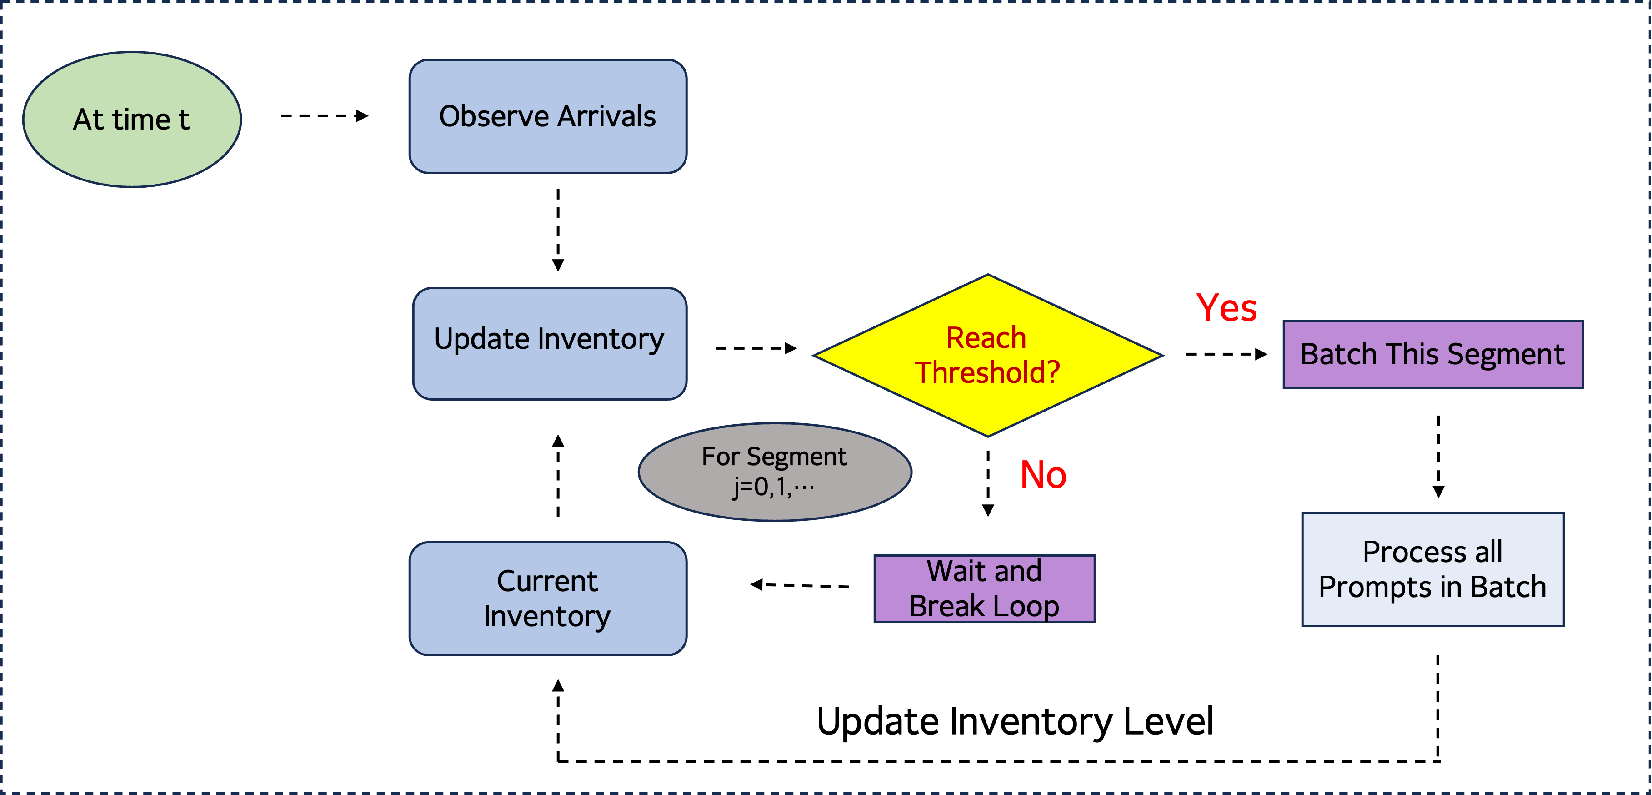
\includegraphics[width=0.9\linewidth]{Experiments_pdf/fig_nestedWAIT.pdf}
    \caption{Pipeline of the Nested WAIT Algorithm}
    \label{fig:nested_wait}
\end{figure}
Consider Example~\ref{ex:unknown_output} with two prompt types: ``Hello'' $\to$ ``Hi'' (1 token, type 1) and ``Hello'' $\to$ ``Hi there!'' (2 tokens, type 2). At arrival, we cannot distinguish them. After one decode iteration, however, \textbf{the prompts reveal themselves}: type-1 prompts have completed their output (``Hi'') and exit; type-2 prompts have generated only their first token (``Hi'') and continue. Nested WAIT exploits this revelation by partitioning processing into two segments. \textbf{Segment 1} processes all newly arrived prompts (both types) through stages $0, 1$ (up to $l_1'=1$) at combined rate $\lambda_1 + \lambda_2$. \textbf{Segment 2} processes only type-2 prompts (those that survived segment 1) through stage $2$ (up to $l_2'=2$) at reduced rate $\lambda_2$. \textbf{No prediction is needed}—prompts simply classify themselves by completing or continuing at the segment 1 boundary.

Figure~\ref{fig:nested_wait_example} visualizes the algorithm in action. At time \( t=0 \), prompts \( P1 \) and \( P2 \) arrive but are insufficient to trigger processing, as Segment 1 has fewer than 3 prompts. At \( t=1 \), \( P3 \) arrives, satisfying the Segment 1 threshold, and the batch is processed. Since these prompts have just begun decoding, none qualify for Segment 2. At \( t=5 \), a new wave of prompts (\( P4 \), \( P5 \)) arrives, again below the threshold. By \( t=7 \), the threshold is met with \( P6 \), \( P7 \), and processing proceeds. Now, \( P3 \), having reached a deeper decode stage, transitions to Segment 2. However, since the Segment 2 threshold is still unmet, only Segment 1 is processed. Finally, at \( t=14 \), enough prompts have advanced into Segment 2 (\( P3 \), \( P5 \), \( P6 \), etc.) to satisfy both segment thresholds. At this point, the Nested WAIT algorithm jointly schedules both segments, batching according to type-specific readiness. This example shows how the algorithm defers processing to ensure type separation and stage-aligned batching.


\begin{figure}[h]
    \centering
    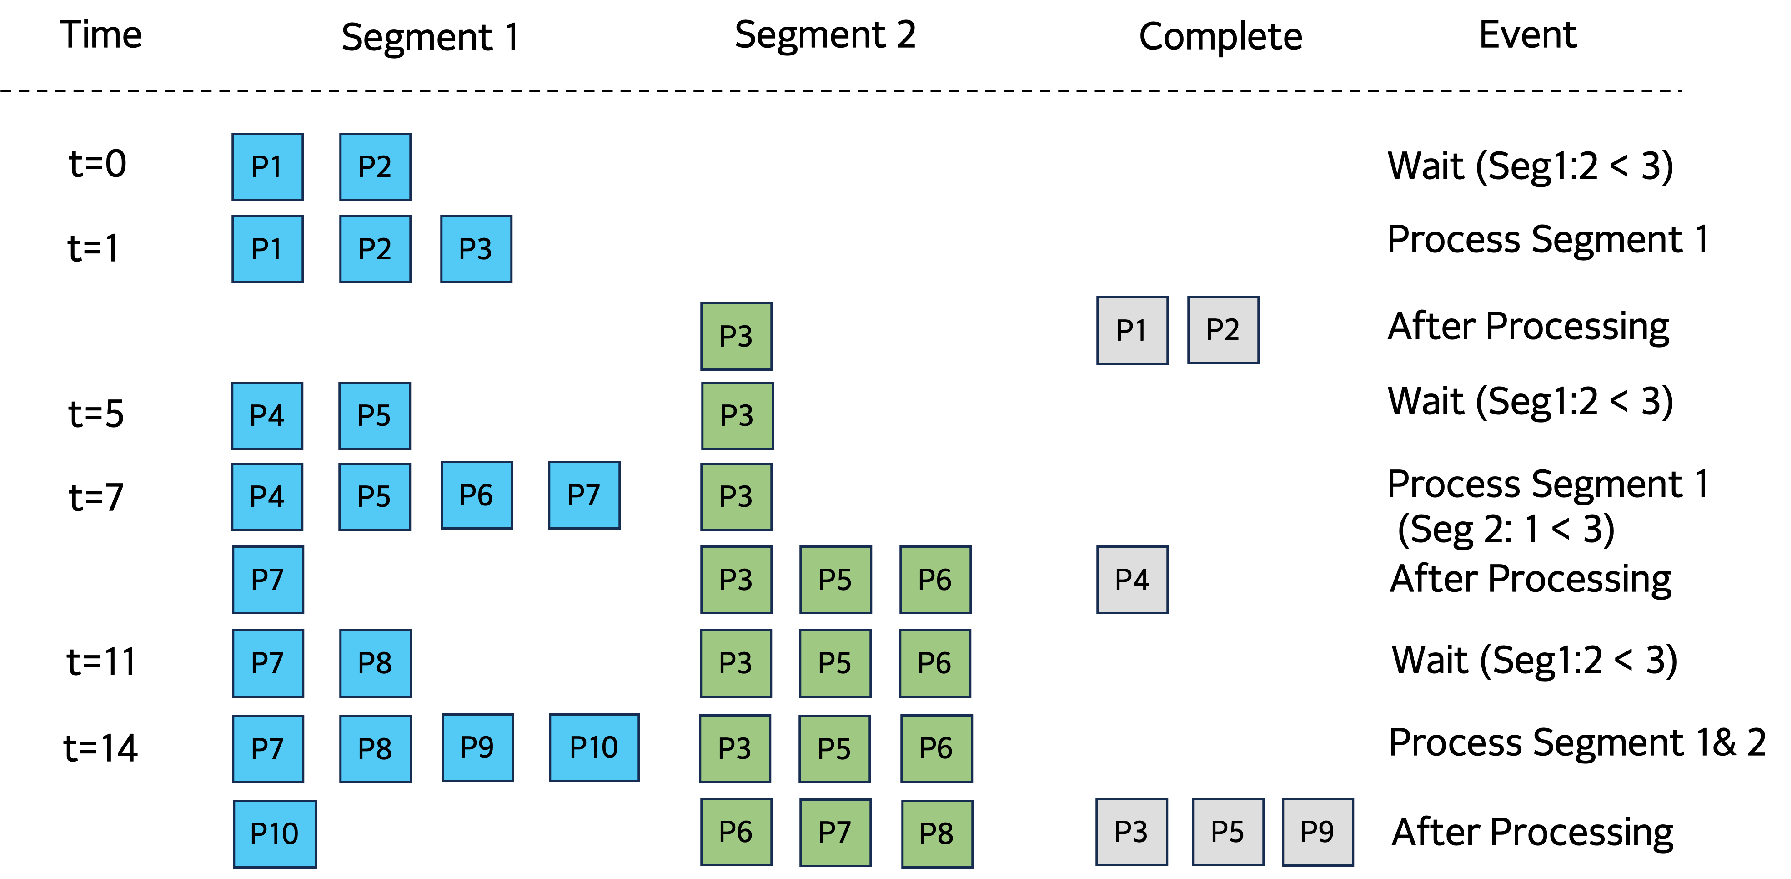
\includegraphics[width=0.9\linewidth]{Experiments_pdf/fig_nestedWAIT_example.pdf}
    \caption{Example of the Nested WAIT Algorithm}
    \label{fig:nested_wait_example}
\end{figure}

\begin{algorithm}[h]
\caption{Nested WAIT: Nested Waiting for Accumulated Inference Threshold}
\label{alg:nested_wait}
{\small\linespread{1.0}\selectfont
\begin{algorithmic}[1]
\Require Memory capacity \( C \), arrival rates \( \lambda_j \) for \( j \in [m] \), thresholds \( n_k \) for segments \( k \in [m] \)
\Require Output lengths \( l_1' < l_2' < \cdots < l_m' \) for prompt types \( j \in [m] \)
\Statex \Comment{$Q_{k,s}$: number of prompts in segment $k$ at decode stage $s$; entry stage of segment $k$ is $l_{k-1}'$ (with $l_0'=0$)}
\State Initialize \( Q_{k,s} \gets 0 \) for all segments \( k \in [m] \) and stages \( s \in [l_{k-1}', l_k'-1] \)
\State Initialize event queue; set current time \( t \gets 0 \)
\While{True}
    \State Wait for the next event (arrival or batch completion)
    \If{event is an arrival}
        \State \( Q_{1,0} \gets Q_{1,0} + 1 \)  \Comment{New prompts enter segment 1 at stage 0}
    \ElsIf{event is a batch completion for segment \( k \)}
        \For{each stage \( s \) in segment \( k \)}
            \State Advance \( \min\{n_k, Q_{k,s}\} \) prompts from stage \( s \) to \( s+1 \)
        \EndFor
        \If{prompts reach stage \( l_k' \) (end of segment $k$)}
            \If{\( k < m \)}
                \State Move to segment \( k+1 \) at stage \( l_k' \) \Comment{These are type-$(k+1)$ or longer}
            \Else
                \State Complete and clear KV caches
            \EndIf
        \EndIf
    \EndIf
    \State Find largest \( k \) such that \( Q_{k', l_{k'-1}'} \geq n_{k'} \) for all \( k' \leq k \) \Comment{All segments up to $k$ meet threshold}
    \If{such \( k \) exists}
        \State Form batch from segments \( 1, \dots, k \): select \( \min\{n_{k'}, Q_{k',s}\} \) prompts per stage
        \State Process batch; prompts outside batch wait with KV caches retained
    \EndIf
\EndWhile
\end{algorithmic}
}
\end{algorithm}

This nested structure directly implements the four design principles from Example~\ref{ex:unknown_output}: (i) we \textbf{avoid eviction} by never exceeding thresholds; (ii) prompts \textbf{classify on-the-fly} at segment boundaries; (iii) we \textbf{don't waste throughput} because each segment operates at its own optimal threshold; (iv) \textbf{short prompts finish first} within segment 1, freeing memory without waiting for long prompts. Crucially, \textbf{no prediction is needed}—prompts simply reveal their output by completing or continuing. This achieves high memory utilization \textbf{for all types simultaneously}, not just the shortest or longest. We now formalize this intuition.

\subsection{Main Theorem}
\label{subsec:nested_main_theorem}

We now analyze Nested WAIT in the asymptotic regime, following the same framework as Section~\ref{sec:wait}. The unknown-output-length setting introduces \textbf{additional stochastic variability}: since we cannot predict which prompts will be long, some may queue at segment boundaries waiting for thresholds. This affects both memory requirements and throughput guarantees. We characterize average throughput $\throughput^{(\zeta, \pi)}$, latency $\Latency^{(\zeta, \pi)}$, and time-to-first-token $\TTFT^{(\zeta, \pi)}$ under threshold policy $\pi = [n_1, \dots, n_m]$.

Before showing Nested WAIT achieves near-optimal throughput, we establish a lower bound showing that \textbf{some} extra memory beyond $M^*$ is necessary when output lengths are unknown.

\textbf{Intuition:} When memory capacity equals exactly $C = M^*$ (the fluid equilibrium), any algorithm that cannot predict output lengths faces a dilemma at every iteration. If we admit too many prompts optimistically, some will reveal longer outputs than expected, causing overflow and eviction. If we admit too few conservatively, we waste capacity. Either scenario creates a throughput gap of $\Omega(1)$ over time.

\begin{proposition}
\label{prop:unknown_lower_bound}
When memory capacity \( C \) equals the equilibrium memory \( M^* \), there exists an instance where any online non-predictive policy \( \pi \), unaware of prompt types upon arrival, incurs a throughput gap \( \throughput^* - \mathbb{E}[\throughput^{(\zeta, \pi)}] = \Omega(1) \).
\end{proposition}

This lower bound shows that uncertainty has a cost: we need more memory than the fluid equilibrium to hedge against unknown output lengths. Theorem~\ref{thm:nested_wait_heavy_traffic} shows that only a \textbf{logarithmic} amount of extra memory suffices under Nested WAIT.
% See Appendix \ref{sec:proof_unknown_lower_bound} for a detailed proof.



As in Section~\ref{sec:wait}, thresholds must balance two goals: (i) \textbf{throughput efficiency} (don't wait too long to form batches); (ii) \textbf{segment stability} (ensure later segments receive enough prompts). This leads to two constraints, analogous to Equation~\eqref{eq:wait_thresholds}.

Similar to Equation \eqref{eq:wait_thresholds}, we define \( \Delta T_{[1,\dots,m]}(n_1, \dots, n_m) \) as the time cost per iteration with exactly \( n_k \) prompts per stage in segment \( k \), for all \( k \in [1, \dots, m] \). Thresholds must satisfy:
\begin{equation}
    \label{eq:nested_wait_thresholds}
    \begin{aligned}
    &\Delta T_{[1,\dots,m]}(n_1, \dots, n_m) <\frac{n_1}{\sum_{j=1}^m \lambda_j}, \\
    &\frac{n_{k+1}}{n_k} > p_k,\forall k \in \{1, \dots, m-1\},
    \end{aligned}
\end{equation}
where $p_k = (\sum_{j=k+1}^m\lambda_j)/(\sum_{j=k}^m\lambda_j)<1.$ To state the memory requirement, we define the memory usage when running iteration with exactly \( n_k \) prompts per stage in segment \( k \), for all \( k \in [1, \dots, m] \) as:
\begin{equation}
    \label{eq:nested_wait_memory}
\begin{aligned}
        M^\pi &= \sum_{k=1}^m n_k \big(l + \tfrac{1}{2}L_k'\big) \Delta l_k', \\
    &\text{where } L_k' = \sum_{r=1}^k l_r',\ \Delta l_k' = l_k' - l_{k-1}',\ l_0' = 0.
\end{aligned}
\end{equation}
Here, the formula captures the peak batch memory when exactly $n_k$ prompts occupy each segment $k$: the term $n_k$ is the threshold (maximum prompts concurrently decoding in segment $k$), $\Delta l_k' = l_k' - l_{k-1}'$ counts the decode stages spanned by segment $k$, and $(l + \tfrac{1}{2}L_k')$ represents the average memory per prompt within segment $k$, where $L_k' = l_1' + \cdots + l_k'$ is the cumulative decode length.
We define the total number of iterations over time horizon $[0,T]$ as $B$. Therefore, we have $T\ge\sum_{b=1}^B \Delta T_{b\text{-th Batch}}\geq B\cdot \min \Delta T_{\text{Batch}}$, where $\Delta T_{b\text{-th Batch}}$ denotes the time cost of the $b$-th iteration and $\Delta T_{\min}=\min_b\{\Delta T_{\text{Batch}}\}$.
Theorem~\ref{thm:nested_wait_heavy_traffic} establishes asymptotic optimality for Nested WAIT in the asymptotic regime with unknown prompt types, given thresholds \( \pi = [n_1, \dots, n_m] \) satisfying Equation \eqref{eq:nested_wait_thresholds}.

\begin{theorem}
\label{thm:nested_wait_heavy_traffic}
Assume thresholds \( \pi = [n_1, \dots, n_m] \) satisfy Equation \eqref{eq:nested_wait_thresholds}, and memory \( M \) satisfies:
\begin{equation}
    \label{eq:nested_wait_memory_total}
\begin{aligned}
    &M^{(\zeta,\pi)}\\
\geq &M^\pi + \sum_{k=2}^m (l + l_{k-1}') \bigg(n_k + \theta_k^{-1} \ln\Big( \frac{m \zeta B}{\delta} \Big)\bigg) \\
=& O\bigg( 2M^\pi + \sum_{k=1}^m (l + l_{k-1}') \theta_k^{-1}\ln\Big( \frac{m \zeta B}{\delta} \Big) \bigg),
\end{aligned}
\end{equation}
where $\theta_k \geq 8(n_k - n_{k-1}p_k)/n_k.$ Then:
$$
    \begin{aligned}
        &\throughput^* - \mathbb{E}\big[ \throughput^{(\zeta, \pi)} \big] 
   = O\big( (\zeta T)^{-1} \big), \\
&\mathbb{E}\big[ \Latency^{(\zeta, \pi)} \big],\,\mathbb{E}\big[ \TTFT^{(\zeta, \pi)} \big] = O(1).
    \end{aligned}
$$
Moreover, memory is not exceeded with probability at least \( 1 - \delta \) during time horizon $[0,T].$
% over the total batch counts $s\in \{1,\cdots,S\}$ as well as the time horizon $t \in [0, T]$, where $T=\sum_{i=1}^S \Delta T_{i\text{-th Batch}}\geq S\cdot \min \Delta T_{\text{Batch}}$.
\end{theorem}

Nested WAIT extends the dimensionality reduction approach from WAIT to handle unknown output lengths. The core insight is that thresholds $n_k$ in each segment $k$ bound the state space, just as in WAIT—but now prompts classify themselves on-the-fly by completing or continuing at segment boundaries, rather than revealing their type at arrival. There is even no need to know the actual output—we only observe whether each prompt completes or continues. This on-the-fly classification creates a key technical challenge: prompts entering segment 2 at time $t$ are precisely those that survived segment 1, creating a delayed arrival process with rate $\lambda_2 + \cdots + \lambda_m$ that depends on the history of earlier segments. We address this through a coupling argument: the number of prompts transitioning from segment $k$ to $k+1$ couples to a Poisson process with rate $\sum_{j=k+1}^m \lambda_j$, allowing us to analyze each segment's queue independently despite the temporal dependency.

This coupling reveals why the safety buffer is necessary. When segment $k$ has fewer than $n_k$ prompts, processing pauses and prompts queue at the boundary. Because we cannot predict which prompts will advance to later segments, this queueing introduces stochastic fluctuations beyond the fluid limit. Doob's maximal inequality bounds the maximum queue length over time horizon $[0, T]$ with high probability, showing the bound grows only as $O(\ln(T/\delta))$—this logarithmic overhead is the safety buffer in Equation~\eqref{eq:nested_wait_memory_total}. The key is that despite not knowing output lengths, the threshold mechanism keeps each segment close to its equilibrium batch size, maintaining the system near the load-balanced state where arrivals match completions. This prevents the cascading evictions that occur in FCFS (Example~\ref{ex:fcfs_cascade}) while achieving the same design goals as WAIT: eviction prevention, approaching load balance, and memory exploitation. The full proof in Appendix~\ref{appendix::proof of nested_wait_heavy_traffic} formalizes the coupling construction and derives explicit constants.

The memory requirement in Equation~\eqref{eq:nested_wait_memory_total} consists of two components with clear operational interpretations:

\begin{enumerate}
    \item \textbf{Base memory $M^\pi$}: This is the equilibrium memory from the fluid model---the memory needed when exactly $n_k$ prompts occupy each stage in segment $k$. This represents the ``steady-state'' memory consumption.

    \item \textbf{Safety buffer} $\sum_{k=2}^m (l + l_{k-1}')(n_k + \theta_k^{-1}\ln(m\zeta B/\delta))$: This additional memory hedges against stochastic fluctuations when output lengths are unknown. It has three components:
    \begin{itemize}
        \item $n_k$: Accounts for prompts queueing at segment $k$ boundaries, waiting for thresholds.
        \item $\theta_k^{-1}\ln(m\zeta B/\delta)$: High-probability protection against queue buildup (overflow occurs with probability $\leq \delta$).
        \item $(l + l_{k-1}')$: Memory footprint of prompts at the boundary between segments $k-1$ and $k$.
    \end{itemize}
\end{enumerate}

This safety buffer is \emph{logarithmic} in the time horizon $T$ (via $B$) and confidence level $1/\delta$, making it a modest overhead compared to the base memory $M^\pi$. This is why Proposition~\ref{prop:unknown_lower_bound} shows that \emph{some} extra memory beyond $M^*$ is necessary for unknown output lengths, but our Theorem~\ref{thm:nested_wait_heavy_traffic} demonstrates that only a logarithmic amount suffices.

\textbf{Number of types:} The algorithm's performance depends primarily on arrival rates and output lengths, not the number of types $m$. Even for large $m$ (e.g., output lengths $\{1, 2, \dots, m\}$), descending thresholds $n_1 > n_2 > \dots > n_m$ remain effective when arrival rates satisfy condition~\eqref{eq:nested_wait_thresholds}.

\textbf{Safety buffer overhead:} The memory requirement in~\eqref{eq:nested_wait_memory_total} is typically dominated by the base term $M^\pi$. The safety buffer (second term) grows only logarithmically in the time horizon and is modest in practice. Section~\ref{sec:numerical} provides numerical validation.

\textbf{Segment-wise generalization:} In practice, we use a \textbf{segment-wise variant} that groups $m$ types into $L \leq m$ segments (Section~\ref{sec:extension}). This design addresses two concerns: (i) robustness to varying or uncertain type distributions; (ii) for long decode lengths, maintaining separate thresholds for every type may be infeasible. Grouping into segments provides stable scheduling with similar guarantees. Having established theoretical foundations for both known and unknown output lengths, we now validate our algorithms experimentally (Section~\ref{sec:numerical}).
% Additional discussion on this generalization is presented in Appendix~\ref{sec:extension}.